\documentclass[conference]{IEEEtran}

\IEEEoverridecommandlockouts                              % This command is only needed if 
                                                          % you want to use the \thanks command

\overrideIEEEmargins                                      % Needed to meet printer requirements.

% See the \addtolength command later in the file to balance the column lengths
% on the last page of the document

\usepackage{amssymb}
\setcounter{tocdepth}{3}
\usepackage{graphicx}
\usepackage[fleqn]{amsmath}
\usepackage{url}
\usepackage{amsmath} % assumes amsmath package installed
\usepackage{amssymb}  % assumes amsmath package installed
\usepackage{algorithm}			% pacchetti per i pezzi di pseudocodice
\usepackage{algorithmic}		% pacchetti per i pezzi di pseudocodice

\usepackage{float}		% pacchetto per figure e tabelle


%\usepackage{mathptmx} % assumes new font selection scheme installed
%\usepackage{times} % assumes new font selection scheme installed


% correct bad hyphenation here
\hyphenation{op-tical net-works semi-conduc-tor}


\begin{document}
%
% paper title
% can use linebreaks \\ within to get better formatting as desired
\title{ART@Work: Team Description Paper}



\author{\IEEEauthorblockN{Marco Imperoli\IEEEauthorrefmark{1},
Michele Marostica\IEEEauthorrefmark{2},
Nicolò Boscolo\IEEEauthorrefmark{2}
Roberto Capobianco\IEEEauthorrefmark{1} and 
Jacopo Serafin\IEEEauthorrefmark{1}}\\
\IEEEauthorblockA{\IEEEauthorrefmark{1}Department of Computer, Control, and Management Engineering\\``Antonio Ruberti``, Sapienza University of Rome, Italy.\\ Email: {\tt\small marcoimperoli@gmail.com, {serafin,capobianco}@dis.uniroma1.it}}
\IEEEauthorblockA{\IEEEauthorrefmark{2}Department of Information Engineering, University of Padova, Italy.\\ Email: {\tt\small michelemaro@gmail.com, nicolo.boscolo@it-robotics.it}}}

% make the title area
\maketitle


\begin{abstract}
%\boldmath
The abstract goes here.
\end{abstract}

\section{Introduction}
% no \IEEEPARstart
This demo file is intended to serve as a ``starter file''
for IEEE conference papers produced under \LaTeX\ using
IEEEtran.cls version 1.7 and later.

Test citation \cite{thrunburgardfox2005}.\\
Test Image in Fig.~\ref{fig:test_img}.\\
\begin{figure}[t!]
\begin{center}
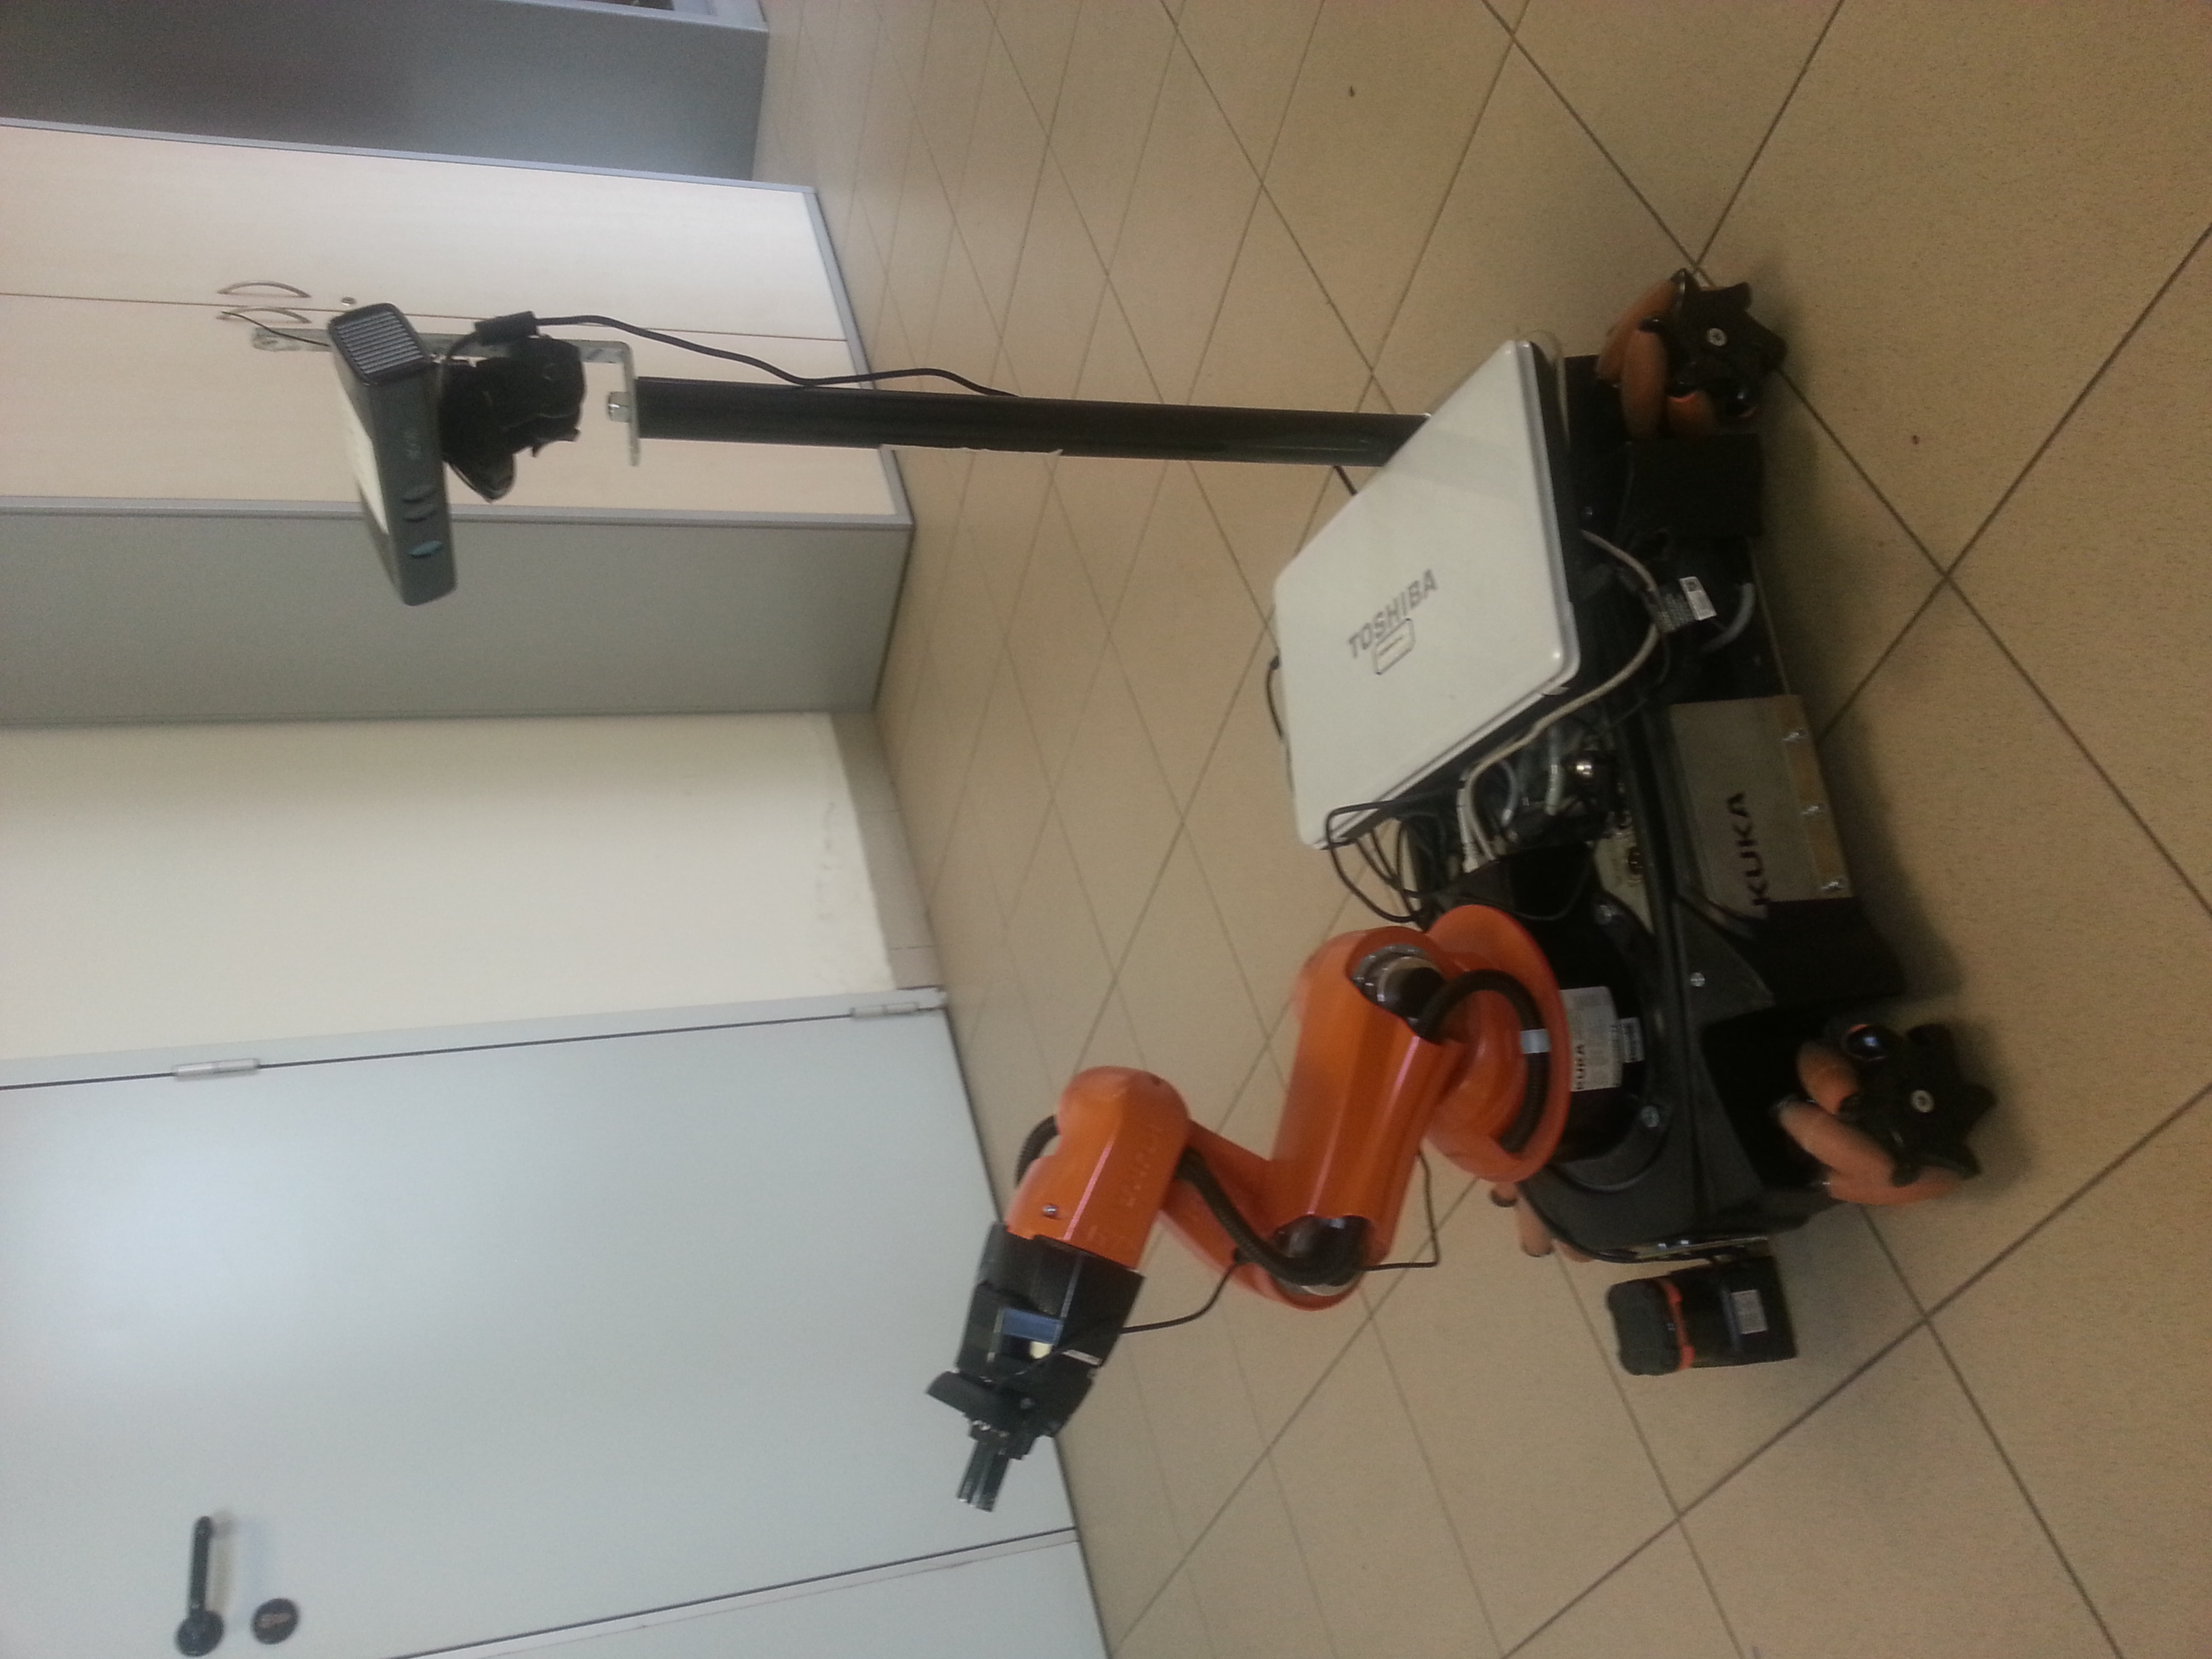
\includegraphics[angle=0,width=\linewidth]{images/test_img.png}
\end{center}
\caption{Test image.}\label{fig:test_img}
\end{figure}

\subsection{Subsection Heading Here}
Subsection text here.


\subsubsection{Subsubsection Heading Here}
Subsubsection text here.



\section{Conclusion}
The conclusion goes here.

\bibliographystyle{IEEEtran}
\bibliography{bibliography} 

% that's all folks
\end{document}


